
\section{The algorithm}
\label{sec:algorithm}
\comment{Mettiamo PS algorithm come titolo della sezione almeno rinforziamo nella memoria il suo nome?}
In this section we present PS, the algorithm that we propose to perform the Design Space Exploration (DSE). As any other DSE algorithm, its input is the parameterized system $S$ and a benchmark application $b$, while the output is an approximation of the Pareto-optimal set $\mathcal{P}\left(S,b\right)$. \comment{E' corretto?}  
PS is iterative and we will describe, separately, the initialization phase, the operations performed inside each iteration and the condition that triggers the termination.

By a slightly abuse of notation, considering a subset $I$ of the configuration space, we will denote with $\mathcal{P}(I,b)$ the non-dominated feasible configurations in $I$, i.e.
	\begin{align}
		\mathcal{P}(I,b)=
		\left\{ \mathbf{c} \in I \cap \mathcal{C}^*(S) | \nexists \ \mathbf{c}' \in I \cap \mathcal{C}^*(S), \mathbf{c}' \succ \mathbf{c} \right\}
	\end{align}
Since in each run of the algorithm we will consider only one benchmark application $b\in\mathcal{B}$, we will omit it, replacing, for example, $\mathcal{P}(I,b)$ with  $\mathcal{P}(I)$.

Each iteration is called \emph{era}. The $i$-th era is characterized by: 
	\begin{itemize}
	\item the set of regions $\mathcal{R}_{i}$ in which the configuration space
	$mathcal{C}(S)=V_{1}\times\dots\times V_{n}$ is partitioned
	\item an approximation $\mathscr{P}_{i}$ of the Pareto-optimal set.
	\item a set $test_{i}$ of at most $K$ configurations evaluated in the era. \comment{Nella era i o nella successiva?}
	\end{itemize}
$K$ is a parameter that must be set before the algorithm runs. \comment{Spiegare un po' l'impatto di K.} Note that $\mathcal{R}_{i}$ is a partition of the configuration space, i.e.
	\begin{align}\begin{array}{l}
		\bigcup_{R\in\mathcal{R}_i} R = \mathcal{C}(S) \mbox{ and}\\
		R' \cap R'' = \emptyset, \forall R',R'' \in \mathcal{R}_i
	\end{array}\end{align}

\comment{Prima di sbattere tutta la sfilza di steps, dovremmo dare un'idea preliminare di cosa si andra' a fare.}

\subsection{Initialization}
We fix $\mathcal{R}_0$, $\mathscr{P}_0$ and $test_0$ for the era $0$ as follows. Era $0$ has only one region that is the whole parameter space,
i.e. $\mathcal{R}_{0}=\left\{ V_{1}\times\dots\times V_{n}\right\} $.
A random set $test_{0}$ of $K$ configurations is evaluated. The
Pareto set $\mathscr{P}_{0}=\mathscr{P}\left(test_{0}\right)$ is
calculated.



\subsection{Iteration steps}

For $era_{i}$ with $i>0$ the following operations must be performed.
\begin{enumerate}
\item \label{pers02.enu:K}
In each era $i$, a set $test_i$ of $K$ configurations will be evaluated. We call them \emph{test configurations} and selecting them is exactly the goal of this step.
We select only \emph{new} configurations, i.e. the ones that have not been evaluated in past eras. In other words, $test_i$ must not contain $\bigcup_{j=0}^{i-1}test_{j}$.
Since all regions $R$ in the configuration space partition $\mathcal{R}_{i}$ must be properly explored, we have to distribute the test configurations among all these regions. For this reason, $\frac{K}{\left|\mathcal{R}_{i}\right|}$ configurations are randomly extracted from the new configurations of each region $R\in\mathcal{R}_{i}$. We denote the set of the selected configurations with $test_{R,i}$ and, obviously, $\bigcup_{R\in\mathcal{R}_{i}} test_{R,i} = test_i$.
 In case the new configurations in $R$ are less then $\frac{K}{\left|\mathcal{R}_{i}\right|}$, all of them are selected. In this case $test_{R,i}=R\setminus\bigcup_{j=0}^{i-1}test_{j}$, where  $\bigcup_{j=0}^{i-1}test_{j}$ is the set of the configurations already in the past.\footnote{Note that if such regions exist, the total number of evaluations in era $i$ will be less than $K$}
\item All configurations on $test_{i}$ are simulated.
\item The Pareto set $\mathscr{P}_{i}$ for $era_{i}$ is defined as the set of non-dominated configurations among the ones evaluated so far, i.e.
	\[
	\mathscr{P}_{i} \triangleq
	\mathscr{P}\left(\bigcup_{j\leq i}test_j\right)=
	\mathscr{P}\left(test_{i}\cup\mathscr{P}_{i-1}\right)
	\]
where the last equality can easily be proved.

\item \label{pers02.enu:novelty_score_of_a_configuration}
The test configurations that are dominated, i.e. do not belong to $\mathscr{P}_i$, are neglected, while an \emph{innovation score} is given to the other ones, computed on the base of their separation from the non-dominated configurations of the past eras. Recalling that $s$ is the separation (see \defR{separation}), the innovation score of a non-dominated test configuration $\mathbf{c}^*$ is defined as
	\[
	is\left(\mathbf{c}^*\right)=\min\left\{ \left.s\left(\mathbf{c}\rightarrow\mathbf{c} \right)\right|\mathbf{c}\in\mathscr{P}_{i-1}\right\} 
	\]
In other words, a configuration $\mathbf{c}^*$ is characterized by as much innovation
as more separated it is from the configurations of the previous era.

\item Every region $R\in\mathcal{R}_{i}$ is given an innovation score defined
as the sum of the innovation scores of its non-dominated test configurations:
	\[
	is\left(R\right)=\sum\left\{ \left.is\left(\mathbf{c}\right)\right|\mathbf{c}\in\mathscr{P}_{i}\cap R\right\} 
	\]

\item The total innovation and average score for the entire era is calculated:
	\[
	is_{TOT,i}=\sum_{R\in\mathcal{R}_{i}}is\left(R\right)
	\]


\item The configuration space partition $\mathcal{R}_{i}$ is divided in three subsets, that we will comment later \comment{e invece sarebbe bene commentarli ora, anche}:

	\begin{enumerate}
	\item high innovation regions 
	\[
	\mathcal{R}_{i,h}=\left\{ \left.R\in\mathcal{R}_{i}\right|is\left(R\right)>\alpha\cdot is_{av,i-1}\right\} 
	\]
	 where $\alpha$ is a constant defined by the designer (for example
	$\alpha=1.2$). 
	\item low innovation regions 
	\[
	\mathcal{R}_{i,l}=\left\{ \left.R\in\mathcal{R}_{i}\right|0<is\left(R\right)\le\alpha\cdot is_{av,i-1}\right\} 
	\]
	\item no innovation regions 
	\[
	\mathcal{R}_{i,n}=\left\{ \left.R\in\mathcal{R}_{i}\right|is\left(R\right)=0\right\} 
	\]
	\end{enumerate}

\item The goal of this step is preparing the regions that will compose the configuration space partition of the next era, i.e. $\mathscr{R}_{i+1}$. The following operations are performed:
	\begin{enumerate}
		\item Each high innovation region $R\in\mathscr{R}_{i,h}$ is split obtaining $\psi(R)$, as stated in def \defR{splitting-a-region}. We denote with $\psi\left(\mathscr{R}_{i,h}\right)$ the set of regions obtained as explained.
		\item Low innovation regions are left unchanged.
		\item No innovation regions are merged, two by two. To do so, couples of no innovation contiguous regions $(R_1,R_2)$ are selected. We denote the set of these couples as $\mathscr{M}_i$. This set is constructed such that couples are independent, i.e. there cannot be two of them sharing a region. In other words, taking whatever $(R_1,R_2),(R_3,R_4) \in \mathscr{M}_i$, $R_i \neq R_j, \forall i,j\in\lbrace1,2,3,4\rbrace, i\neq$. 
We merge each couple of regions, i.e. $\forall (R_1,R_2)\in\mathscr{M}_i$ we calculate $\mu(R_1,R_2)$, according to \defR{merging-regions}.
We stress that the regions that belong to each selected couple must be contiguous, otherwise it is impossible to merge them. We denote with $\mu(\mathscr{M}_i)$ the set of the merged regions, i.e. $\mu(\mathscr{M}_i) = \bigcup_{(R_1,R_2)\in\mathscr{M}_i} \mu(R_1,R_2)$
	\end{enumerate}


\item The set of regions $\mathcal{R}_{i+1}$ for the following era is computed as:
	\[
	\mathcal{R}_{i+1}=
	\]
	\[
	=\psi\left(\mathscr{R}_{i,h}\right) \cup \mathcal{R}_{i,l}\cup
	\]
	\[
	\cup\left(\mathcal{R}_{i,n}\setminus\bigcup_{\left(R_{1},R_{2}\right)\in\mathcal{C}}\left\{ R_{1},R_{2}\right\} \right)\cup \mu(\mathscr{M}_i)
	\]
\end{enumerate}

\comment{commentare questa formula}

\comment{SONO ARRIVATO A LEGGERE QUA}


\subsection{Termination Condition}
The algorithm terminates at step $k$ if
\[
is_{TOT,k},is_{TOT,k-1},\dots,is_{TOT,k-\beta}\le\gamma\cdot is_{TOT,k-\left(\beta-1\right)}
\]
 where $\beta$ and $\gamma$ are selected by the experimenter (see
remark \ref{rem:termination}).
\begin{remark}
\label{pers02.rem:smaller_regions}The rule \ref{pers02.enu:K} of
the iteration rules says that the smaller is a region, the more ``crowded''
it is. It means that configurations in smaller regions are evaluated
with more ``attention'' (see figure \ref{pers02.fig:small_and_big}).

\begin{figure}[h]
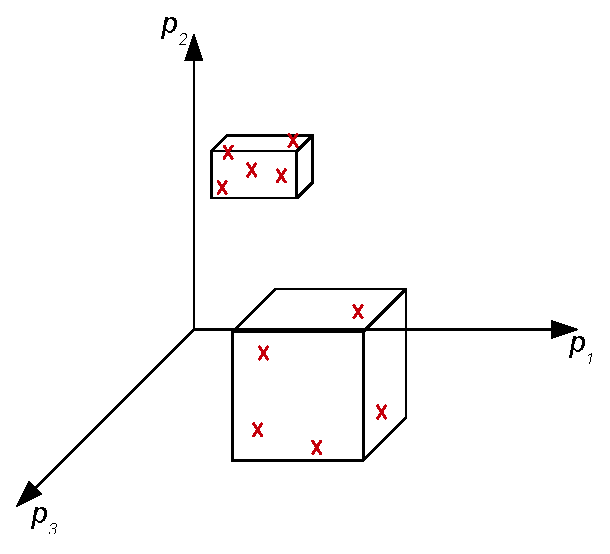
\includegraphics[width=0.5\columnwidth]{img/small_and_big}

\caption{\label{pers02.fig:small_and_big}In this example 5 configurations
are evaluated in a small region and in a bigger region. In can be
seen that smaller region is more crowded.}


\end{figure}

\end{remark}

\begin{remark}
The rule \ref{pers02.enu:novelty_score_of_a_configuration} says that
a configuration whose objectives are more ``separated'' by the previous
Pareto front, has to be taken in greater account than others. A configuration
that is very near, in the objective space, to the previous Pareto
front doesn't add a true innovation. Therefore, the innovation score
of a configuration is a measure of how much interest we have in considering
it (see figure \ref{pers02.fig:Novelty-score-of-a-config}).

\begin{figure}[h]
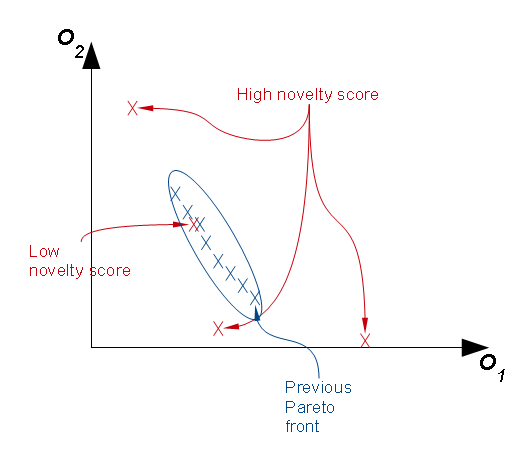
\includegraphics[width=0.5\columnwidth]{img/novelty_score}

\caption{\label{pers02.fig:Novelty-score-of-a-config}innovation score of a
configuration}


\end{figure}

\comment{Ci vorrebbe una rappresentazione schematica dell'algoritmo usando l'ambiente latex Algorithm o non mi ricordo come si chiama}

\end{remark}

\begin{remark}
The innovation score of a region is a measure of how much different
are the points that it adds to Pareto Front compared to the previous
Pareto front. ``High innovation regions'' are the ones in which
more configurations are worth evaluating, because they add many points
on not yet well explored Pareto front areas. Therefore, these regions
are split in the next era (see remark \ref{pers02.rem:smaller_regions})
and more ``crowded'' by simulations. ``No innovation regions''
are the ones that have proved to add few points on Pareto fronts,
probably very near to previous Pareto front points and a Pareto front
point near to previous points is not so much interesting. Therefore
it's not worth evaluating many of their configurations and it is useful
to merge these regions, in order to less densely evaluate them.

%ULTERIORI GIUSTIFICAZIONI SULL'IMPORTANZA DI CONSIDERARE LA DIVERSITA'
%DELLE SOLUZIONI SI TROVA IN ext12.pag5 E ALTRI.

\end{remark}

\begin{remark}
\label{rem:termination}The algorithm terminates when in the last
$\beta$ iterations not a great ``amount of innovation'' has been
discovered. Therefore it is very probably that carrying on iterating
will not considerably change the Pareto front already formed. It's
not recommended to chose $\beta=1$, because it is possible that the
Pareto fronts $\mathbf{o}\left(\mathscr{P}_{k-1}\right)$ and $\mathbf{o}\left(\mathscr{P}_{k}\right)$
are not very different but next Pareto fronts could be. In other words,
it's unsafe to terminate as soon as the Pareto front doesn't change
enough between two consecutive eras, thus a strategy taking into
account the history of the Pareto fronts has been adopted in the
proposed approach.
\end{remark}
%!!! IN INGLESE E' PIU' CORRETTO DIRE: ``IT IS POSSIBLE THAT THE PARETO
%FRONTS WERE NOT VERY DIFFERENT''? (CON ``WERE'' AL POSTO DI ``ARE'')


\begin{remark}
Merging and splitting the regions are very dynamic processes. A portion
of the parameter space can be populated by a large number of small
regions in some eras, but can be covered by a small number of large
regions in next eras. This can be explained saying that, after a number
of eras of intense exploration of a portion of parameter space, this
exploration has turned to be enough thorough and so it was time for
other portions to be minutely scanned.
\end{remark}
